
\chapter{Aufgabe D11}
Zum Driver Model wird ein Error Model hinzugefügt.
\begin{figure}[H]
	\centering
	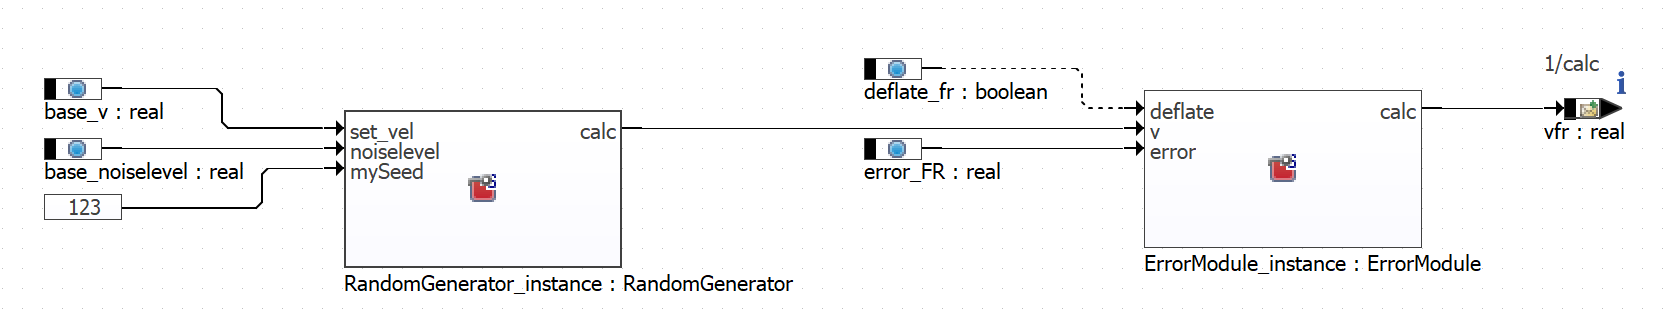
\includegraphics[width=1\linewidth]{../Graphiken/Errorintegration.png}
	\caption{Error Module Integration}
	\label{fig:ErrorModuleIntegration}
\end{figure}
Ist das Error Modul inaktiv leitet es die generierte Geschwindigkeit durch. Wird es aktiviert wird der generierten Geschwindigkeit ein prozentualer Fehler abgezogen.
\begin{figure}[H]
	\centering
	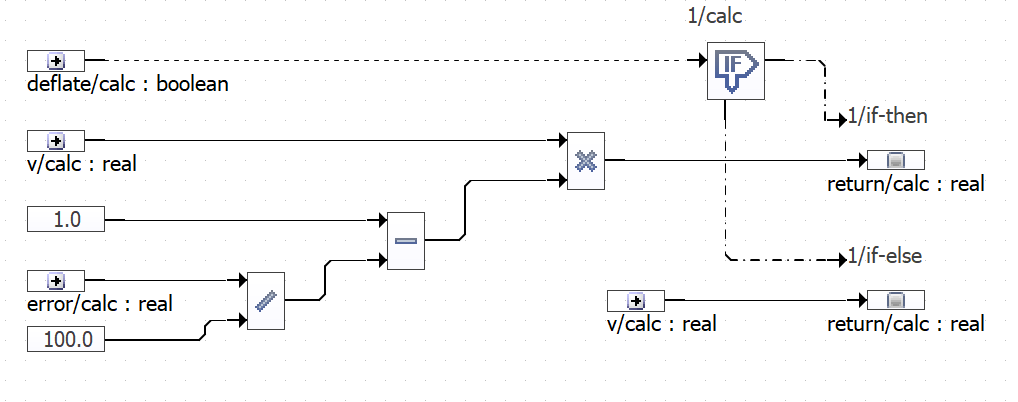
\includegraphics[width=0.85\linewidth]{../Graphiken/ErrorModule.png}
	\caption{Error Module}
	\label{fig:ErrorModule}
\end{figure}

\begin{figure}[H]
	\centering
\includegraphics[width=0.85\linewidth]{../Graphiken/aktiveError.png}
\caption{Reifendruckabfall aktiv}
\label{fig:ErrorModule}
\end{figure}
Hier ist nur ein aktiver Fehler gezeigt, der länger als 10 Sekunden aktiv ist.